\documentclass[12pt]{article}
\usepackage[english]{babel}
\usepackage{graphicx, amsmath, mathtools, listings, color, caption, rotating, subfigure, fullpage, textcomp, enumerate, float}

\newcommand{\iid}{\stackrel{\mathrm{iid}}{\sim}}

\lstset{
	language=R,
	keywordstyle=\bfseries\ttfamily\color[rgb]{0,0,1},
	identifierstyle=\ttfamily,
	commentstyle=\color[rgb]{0.133,0.545,0.133},
	stringstyle=\ttfamily\color[rgb]{0.627,0.126,0.941},
	showstringspaces=false,
	basicstyle=\tiny,
	numberstyle=\scriptsize,
	numbers=left,
	stepnumber=1,
	numbersep=10pt,
	tabsize=2,
	breaklines=true,
	breakatwhitespace=false,
	aboveskip={1.5\baselineskip},
  columns=fixed,
  upquote=true,
  extendedchars=true,
}

\begin{document}
\begin{center}

\end{center}

\section*{Problem 1}
\begin{enumerate}[(a)]
\item \begin{align*}
	R_{tr} ( \hat(\beta ) ) &= \frac{1}{N} \sum_{i=1}^n \left( y_i - \beta^T x_i \right)^2 
			< \frac{1}{N-p} \sum_{i=1}^n \left( y_i - \beta^T x_i \right)^2 = \text{MSE} \\
			& \Rightarrow E(R_{tr}) < E(MSE) = \sigma^2
	\end{align*}
	
\item \begin{align*}
	E ( R_{te}( \hat(\beta ) ) &= 
	\frac{1}{M} E \sum_{i=1}^M \left( \tilde{y_i} - \hat{\beta}^T \tilde{x_i} \right)^2 \\
%
	&= \frac{1}{M} E \left[ \sum_{i=1}^M \left(  \left( \tilde{y_i} - \hat{\beta}^T \tilde{x_i} \right) + \left( \beta^T \tilde{x_i} - \beta^T \tilde{x_i} \right) \right)^2 \right] \\
%	
	&= \frac{1}{M} E \left[ \sum_{i=1}^M \left( \tilde{y_i} - \beta^T \tilde{x_i} \right)^2 + \sum_{i=1}^M \left( \hat{\beta^T} \tilde{x_i} - \beta^T \tilde{x_i} \right)^2 \right] \\
%
	&= \frac{1}{M} E \sum_{i=1}^M \left( \tilde{y_i} - \beta^T \tilde{x_i} \right)^2 +
	\frac{1}{M} E \sum_{i=1}^M \left( \hat{\beta^T} \tilde{x_i} - \beta^T \tilde{x_i} \right)^2 \\
%
	&= \sigma^2 + \text{(something squared)} > \sigma^2
\end{align*}
\item On average, the training set error will be \emph{less} than the testing set error. This has many implications in both prediction and inference.

\item The attached code generates random noise data sets, calculates training and test set risks, then makes a histogram based on 100 simulations. The blue line is $\sigma^2 = 1$, and the red line is the average risk for training and test set.
\begin{lstlisting}
generateData = function(n, m, p){
  #Takes in training and testing sample sizes and number of predictors.
  #Generates simple noise data
  yTrain = rnorm(n) #Responses
  xTrain = matrix(rnorm(n*p), ncol=p) #Predictors
  
  yTest = rnorm(m) #Responses
  xTest = matrix(rnorm(m*p), ncol=p) #Predictors
  list(yTrain=yTrain, xTrain=xTrain, yTest=yTest, xTest=xTest)
}

calcRisks = function(trainTest){
  # Takes in training and testing data in a list.
  #Unrolls into matrices, then calculates
  # the training and testing errors (scalars). Returns a 2-vector.
  yTrain = trainTest$yTrain
  xTrain = trainTest$xTrain
  yTest = trainTest$yTest
  xTest = trainTest$xTest

  #Compute training OLS estimate, get residuals/coeffs from it.
  trainLM = lm(yTrain ~ xTrain)
  trainResid = trainLM$resid
  trainCoeffs = trainLM$coefficients

  #Use training OLS estimates to make testing fits. Compute errors.
  testFits = cbind(rep(1,nrow(xTest)), xTest) %*% trainCoeffs
  testResid = yTest - testFits
  
  riskTrain = 1/length(yTrain) * sum(trainResid^2)
  riskTest = 1/length(yTest) * sum(testResid^2)
  c(riskTrain, riskTest)
}

n = 100 #Train sample size
m = 100 #Test sample size
p = 10 #Number of predictors
nsim = 100 #Number of simulations

simErrors = t(sapply(1:nsim, function(i) calcRisks(generateData(n, m, p))))
par(mfrow=1:2)
hist(simErrors[,1], main='Histogram of Training Risk', xlab='Training Risk')
abline(v = mean(simErrors[,1]), col='red', lwd=4)
abline(v = 1, col='blue', lwd=4)
hist(simErrors[,2], main='Histogram of Testing Risk', xlab='Testing Risk')
abline(v = mean(simErrors[,2]), col='red', lwd=4)
abline(v = 1, col='blue', lwd=4)
\end{lstlisting}
\begin{figure}[H]
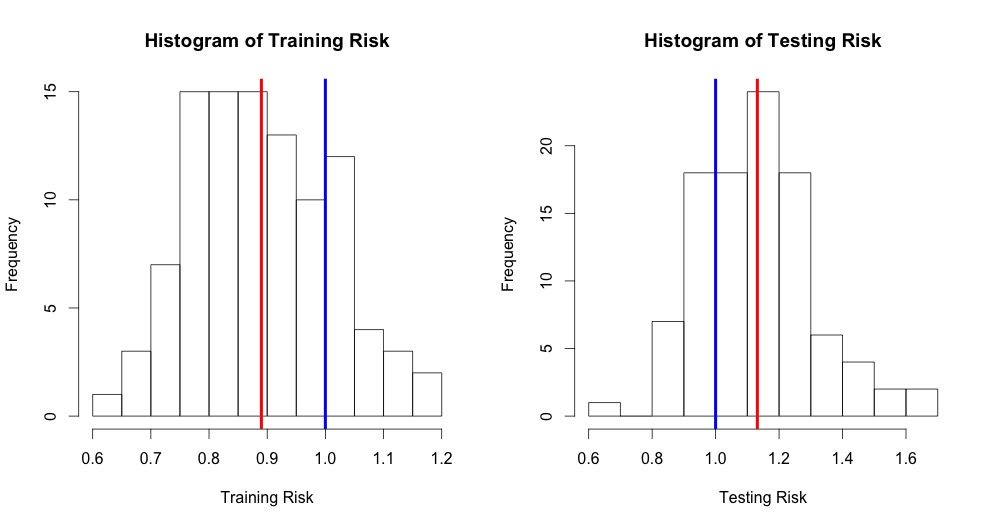
\includegraphics[scale=.4]{RiskHist.jpeg}
\end{figure}
\end{enumerate}

\section*{Problem 2}
\begin{enumerate}[(a)]
\item 
\item 
\end{enumerate}

\section*{Problem 3}
\begin{enumerate}[(a)]
\item A possible rule would be to classify observations to $Y=1$ if $P(Y=1) = \text{sigmoid}(\hat{\beta}^T X) \geq 0.5$. This is equivalent to classifying to $Y=1$ if $\hat{\beta}^T X \geq 0$. Using our logistic regression, classify to $Y=1$ if $0.127 + 0.063 \cdot x_1 + 1.390 \cdot x_2 \geq 0$. The confusion matrix:
\begin{table}[H] \center
\begin{tabular}{ccc} \hline
& Predict 0 & Predict 1 \\ \hline
Actual 0 & 308 &  87 \\ 
Actual 1 & 101 & 304 \\ \hline
\end{tabular}
\end{table}
The misclassification rate is $ (101+87) / 800 = .235$.
\begin{figure}[H]
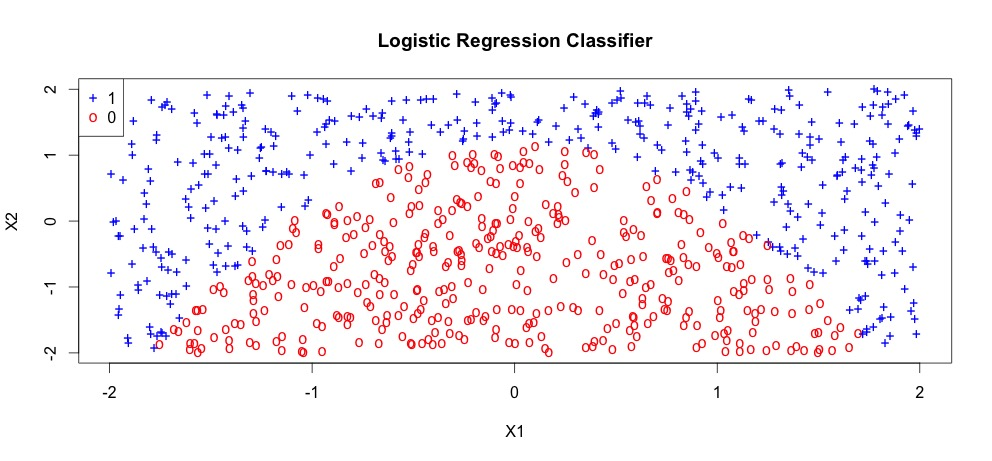
\includegraphics[scale=.4]{y1_plot.jpeg}
\end{figure}

\item Classification rule drawn on the plot, corresponds to the line $x_2 = -0.063 x_1 / 1.390  - 0.127 / 1.390$. This is obtained by taking the classification rule and converting it to slope-intercept form.
\begin{figure}[H]
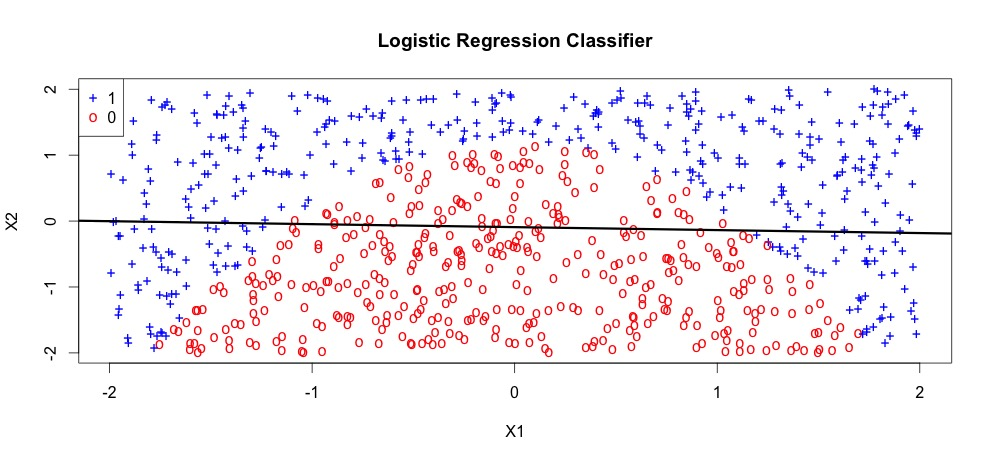
\includegraphics[scale=.4]{y1_plot2.jpeg}
\end{figure}

\item 
\item 
\item 
\item 
\item 
\end{enumerate}

\end{document} 